\chapter{Defining the system}

The simmulated system consist of two major parts: A 2D graphene sheet and a 3D Silicon ``bulk'' substrate. These parts interact with a van der Waals force (modelled by the LJ potential). We apply a normal load to the sheet inducing a normal force response between the sheet and substrate. By dragging the sheet along the substrate we measure the responding frictional forces.
\\
\\
\hl{Maybe include a few words about the preceding considerations between two different simulations approaches: The one that we use now and the \textit{graphene skin} setup, where one would consider the graphene sheet as the top part of the substrate and then measure friction with an indenting tip (AFM-style). This would probably be more directed towards grasping robot applications (with ability to stretch and relax the sheet before grasping) or creation of fixed pre-stretched surfaces in the case that certain friction coefficients of interest could be achieved here.}

\section{Region definitions (Sheet, pullblocks and substrate)}

The system, sheet and substrate, is further subdivided according to
functionality in the MD simmulations. The sheet ends is reserved for so-called
\textit{pull blocks}, which is used application of normal load, stretching and
dragging the sheet, and as a thermostat, while the remaining \textit{inner
sheet} is left as an untouched (NVE) canvas for kirigami cuts. The pull blocks
are equal split between a thermostat part and a rigid part which is locked into
a single rigid body after an initial relaxtion period. Note that the rigid part
of the pull blocks on both side is considered a single rigid object even though
they are physically seperated. This means that all force interactions on these
parts will be applied as a common average making the move in total
synchronization. The substrate is equally divided into three parts: The
\textit{upper layers} (NVE) responsible for the sheet-substrate interaction, the
\textit{middle layers} being a thermostat (NVT), and the \textit{bottom layers}
is frozen (rigid and fixed) in the initial lattice structure to ensure that the
substrate stays in place. In figure \ref{fig:system} the system is displayed
with colors matching the three distinct roles:
\begin{enumerate}
  \item Red: NVE parts which is governing the frictional behaviour of interest.
  \item Green: Thermostats (NVT) sourrounding the NVE parts in order to modify the temperature without making disturbing changes to the interaction of the sheet and substrate.
  \item Blue: Parts that is initially or eventually turned in to rigid objects. For the substrate this is additionally locked off and immobile. 
\end{enumerate}

The total system size in terms of atom count is given in table \ref{tab:system_count} while the sheet length dimension is given in table \ref{tab}

The total system size (without cuts in the sheet) is 27456 atoms, and the distribution into the various regions is shown in table \ref{tab:system_count}. The length dimensions of the sheet is given in table \ref{tab:sheet_dim}.

\begin{figure}[H]
  \centering
  \begin{subfigure}[b]{0.80\textwidth}
      \centering
      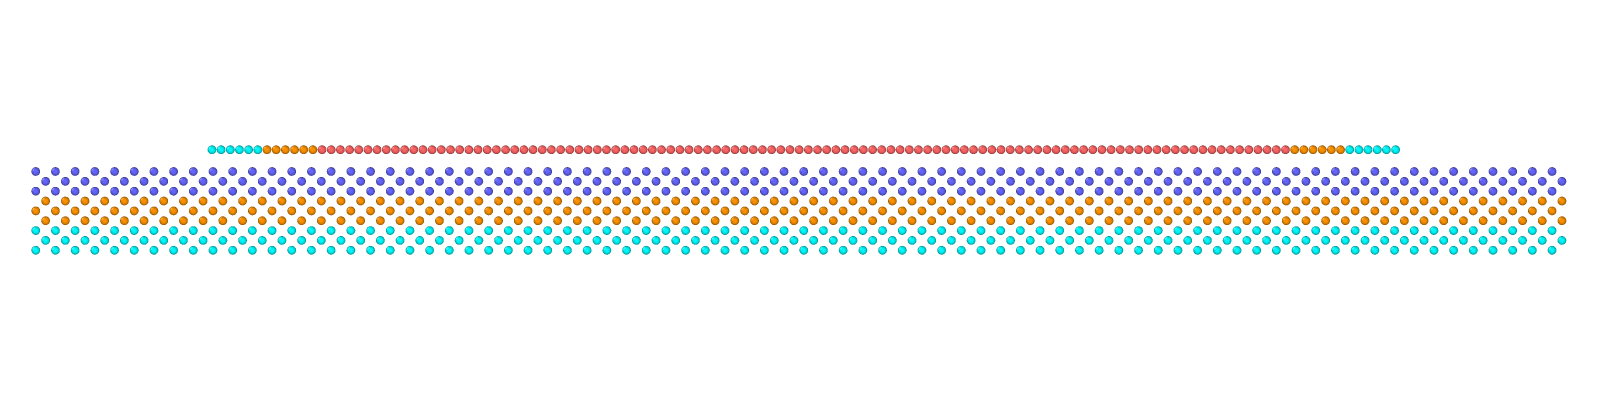
\includegraphics[width=\textwidth]{figures/system/system_sideview.png}
      \caption{Side view showing sheet on top of the substrate.}
      \label{fig:sideview}
  \end{subfigure}
  \hfill
  \begin{subfigure}[b]{0.80\textwidth}
      \centering
      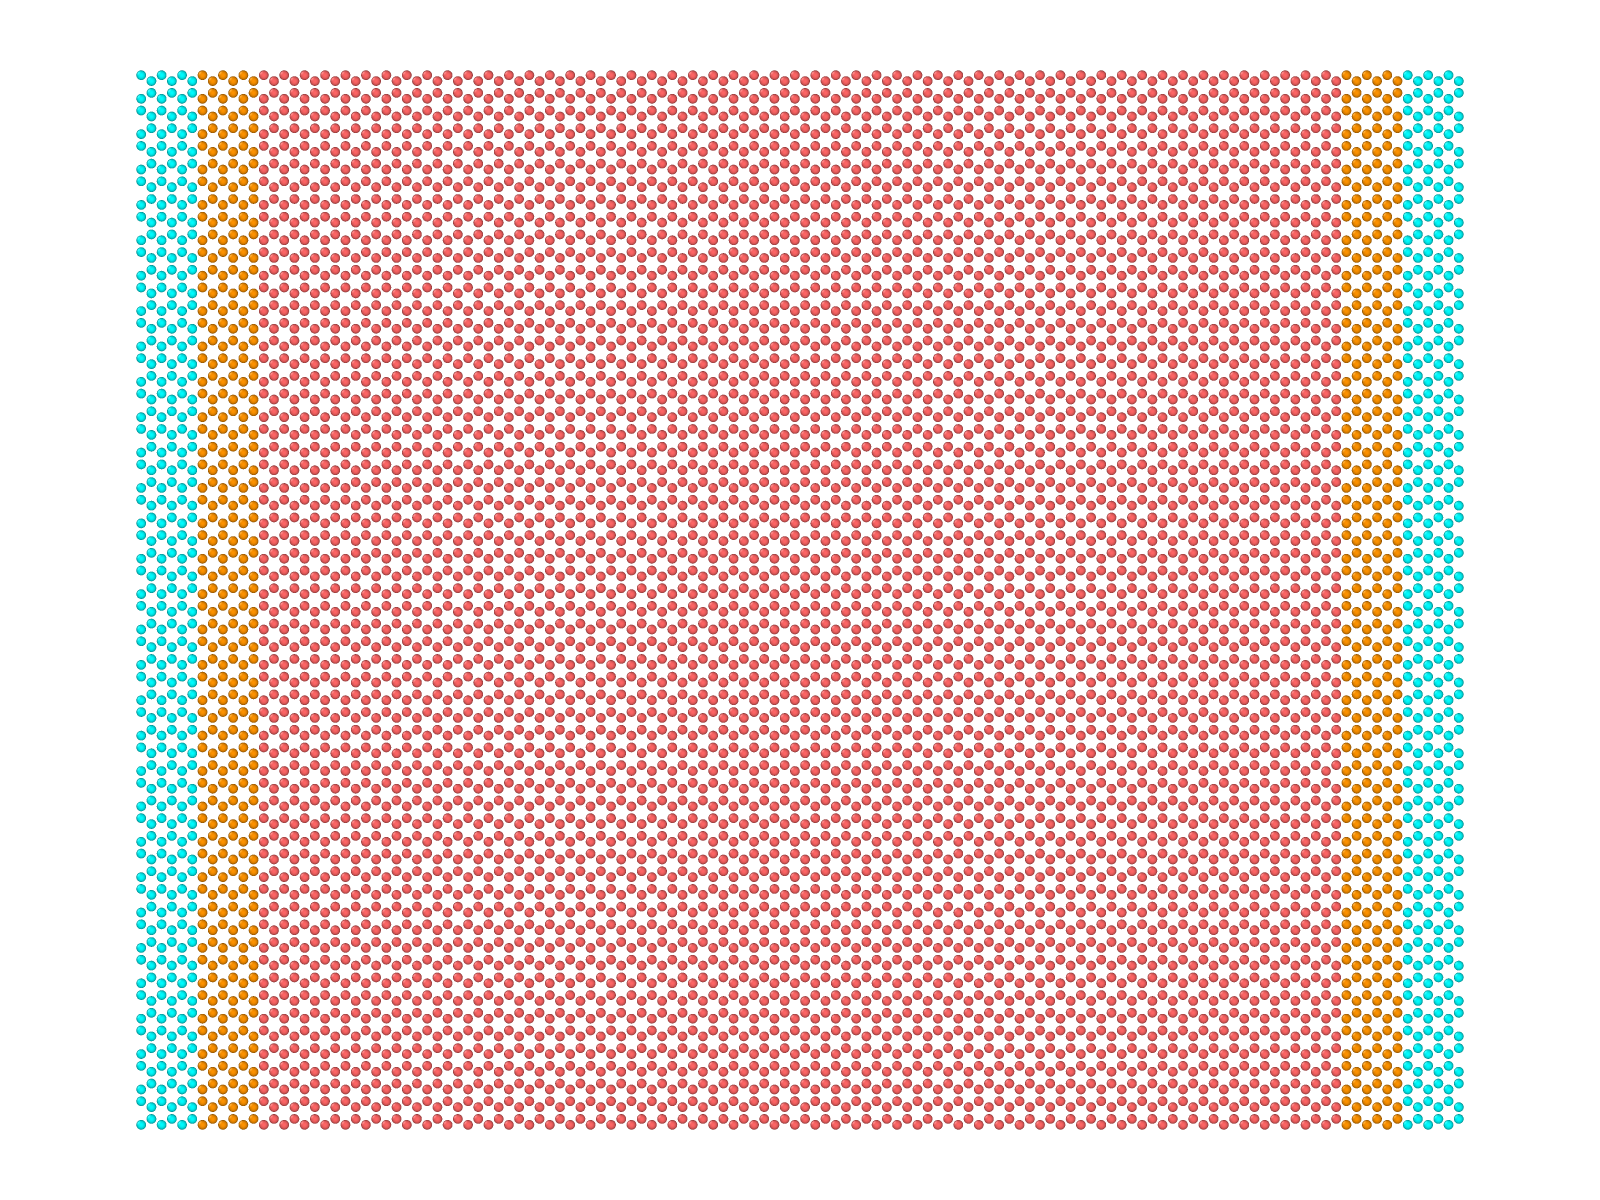
\includegraphics[width=\textwidth]{figures/system/system_topview.png}
      \caption{Top view showing only the sheet.}
      \label{fig:topview}
  \end{subfigure}
  \hfill
     \caption{System configuration colorized to indicate NVE parts (red), thermostat parts (green) and rigid parts (blue).}
     \label{fig:system}
\end{figure}

\begin{table}[H]
  \begin{center}
  \caption{Amount of atoms in the various system regions in the case of no cutting applied to the sheet.}
  \label{tab:system_count}
  \begin{tabular}{ |c|| c | c | c | c | c | c |} \hline
    \textbf{Region} & \textbf{Total}  & Sub region & Sub total & \textbf{NVE} &
    \textbf{NVT} & \textbf{Rigid} \\ \hline   
    \multirow{2}{*}{Sheet} & \multirow{2}{*}{7800} & Inner sheet & 6360 & 6360 &
    0 & 0 \\ %\hline
    & & Pull blocks & 1440 & 0 & 720 & 720 \\ \hline   
    \multirow{2}{*}{Substrate} & \multirow{2}{*}{19656} & Upper & 6552 & 6552 &
    0 & 0 \\ %\hline
    & & Middle & 6552 & 0 & 6552 & 0 \\ %\hline
    & & Bottom & 6552 & 0 & 0 & 6552 \\ \hline \hline   
    All & 27456 & \multicolumn{2}{r|}{} & 12912 & 7272 & 7272 \\ \hline 
  \end{tabular}
  \end{center}
\end{table}


\begin{table}[H]
  \begin{center}
  \caption{Sheet dimensions comparing the full sheet to its subdivisions: inner sheet and pull blocks.}
  \label{tab:sheet_dim}
  \begin{tabular}{ | l | r@{}l | r@{}l | c |} \hline
    \textbf{Group} & \multicolumn{2}{c|}{$x,y$-dim} & \multicolumn{2}{c|}{dim
    [Å]} & Area [Å$^2$]\\ \hline
  Full sheet & $x_S \: \times \: $ & $y_S$ &  $130.029 \: \times \:$ & $163.219$
  Å & $\phantom{2\times} 21,223.203$ \\ \hline
  Inner sheet & $x_S \: \times \:$ & $81.40 \ \%_{y_s}$ &  $130.029  \: \times
  \:$ & $132.853$ Å & $\phantom{2\times} 17,274.743$\\ \hline
  Pull blocks & $2 \times x_S \: \times \:$ & $ \phantom{0}9.30 \ \%_{y_s}$ & $2
  \times 130.029  \: \times \: $ & $\phantom{0}15.183$ Å  & $2 \times
  \phantom{0}1,974.230$ \\ \hline  
  \end{tabular}
  \end{center}
\end{table}


\section{Numerical procedure}

The numerical procedure for the friction simulations can be arranged as the following.

\begin{enumerate}
  \item Relax (15 ps): The sheet and substrate is relaxed for 15 ps. They are
  both initially added in their crystaline form. The sheet is constrained under
  three hard spring forces (spring constant $10^5$ eV/Å$^2$ $\sim$ \num{1.6e6} N/m): One spring
  attathes the sheet center of mass (CM) to its orginal postion preventing
  drift, while the remaining two is attatched to the CM for the pull blocks to
  their initial position respectively to prevent rotation. These spring forces
  are immediately terminated after the relax phase. In this phase the pull
  blocks is only rigid with respect to the z-direction (perpendicular to the
  sheet). That is, all the forces in the z-direction is summed up and
  distributed on the pull blocks while it is free to expand and contract in the
  x-y-plane. This is mainly to ensure that is achieves the correct lattive
  spacing according to the temperature of the system. For the remaining phases
  the rigid parts of the pull block is in fact rigid with respect to all
  directions. 
  \item Stretch: The sheet is stretched by seperating to opposing rigid parts of
  the pullblock at constant velocity until the desired stretch amount is met. 
  \item Pause 1 (5 ps): The sheet is relaxed for 5 ps after the stretch
  procedure.
  \item Pause 2 (Normal load): The normal load is applied to the rigid parts of
  the pull blocks together with a damping force to prevent hard impact between
  sheet and substrate as the seperating distance is now reduced depending on the
  strength of the normal load. The damper is terminated after 0.5 ps, as this
  was suitable for the extreme load cases of our force range, and the system is
  relaxed until a total of 5 ps has passed.
  \item Drag: A virtuel atom is introduced into the simulation which exclusively
  interacts with the rigid parts of the pull through a spring force with variable spring constant $K$ in the x-y-plane. The z-direction is not affected by the spring force and is governed by the balance between normal load and the normal force response from the sheet-substrate interaction. The virtual atom is immediately given a constant velocity corresponding to a variable \textit{drag speed} parameter
\end{enumerate}

At the initial timestep the three nearest neighbours (at distance 1.42 Å) of all graphene atoms is recorded. If these nearest neighbours exceed a threshold of 4 Å this is raises a rupture flag which halt the simulation early. Thus, we effectively prevent any kind of wear on the sheet. For the substrate we do not perform such an analysis but only visually confirms that no wear is accouring under the most extreme simulation parameters. 

\section{Creating the sheet}

We are going to create a 2D sheet graphene sheet. 

\subsection{Graphene}
% (https://community.wvu.edu/~miholcomb/graphene.pdf)
% https://www.physics-in-a-nutshell.com/article/4/lattice-basis-and-crystal

Graphene is a single layer of carbon atom, graphite is the bulk, arranged in a
hexagonallattice structure. We can describe the 2D crystal structure in terms of
its primitive lattice vector and a basis. That is we populate each lattice site
by the given basis and translate it to fill the whole plane by any linear
combination of the lattice vectors
\begin{align*}
  \vec{T}_{mn} = m\vec{a_1} + n\vec{a_2}, \qquad m,n \in \mathbb{N}.
\end{align*}
For graphene we have the primitive lattice vectors 
\begin{align*}
  \vec{a_1} = a \left(\frac{\sqrt{3}}{2}, -\frac{1}{2}\right), \qquad \vec{a_2} = a \left(\frac{\sqrt{3}}{2}, \frac{1}{2}\right), \qquad |\vec{a_1}| = |\vec{a_2} = 2.46 \ \text{Å}.
\end{align*}
Notice that we deliberately excluded the third coordinate as we only consider a
single graphene layer on not the bulk graphite consisting of multiple layers
stacked on top of each other. The basis is 
\begin{align*}
  \Big\{\Big(0,0\Big), \frac{a}{2}\Big(\frac{1}{\sqrt{3}}, 1 \Big) \Big\}
\end{align*}
It turns out that the spacing between atoms is equal for all paris with an
interatomic distance 
\begin{align*}
  \left|\frac{a}{2}\Big(\frac{1}{\sqrt{3}}, 1 \Big)\right| \approx 1.42 \ \text{Å}.
\end{align*}


\begin{figure}[H]
  \centering
  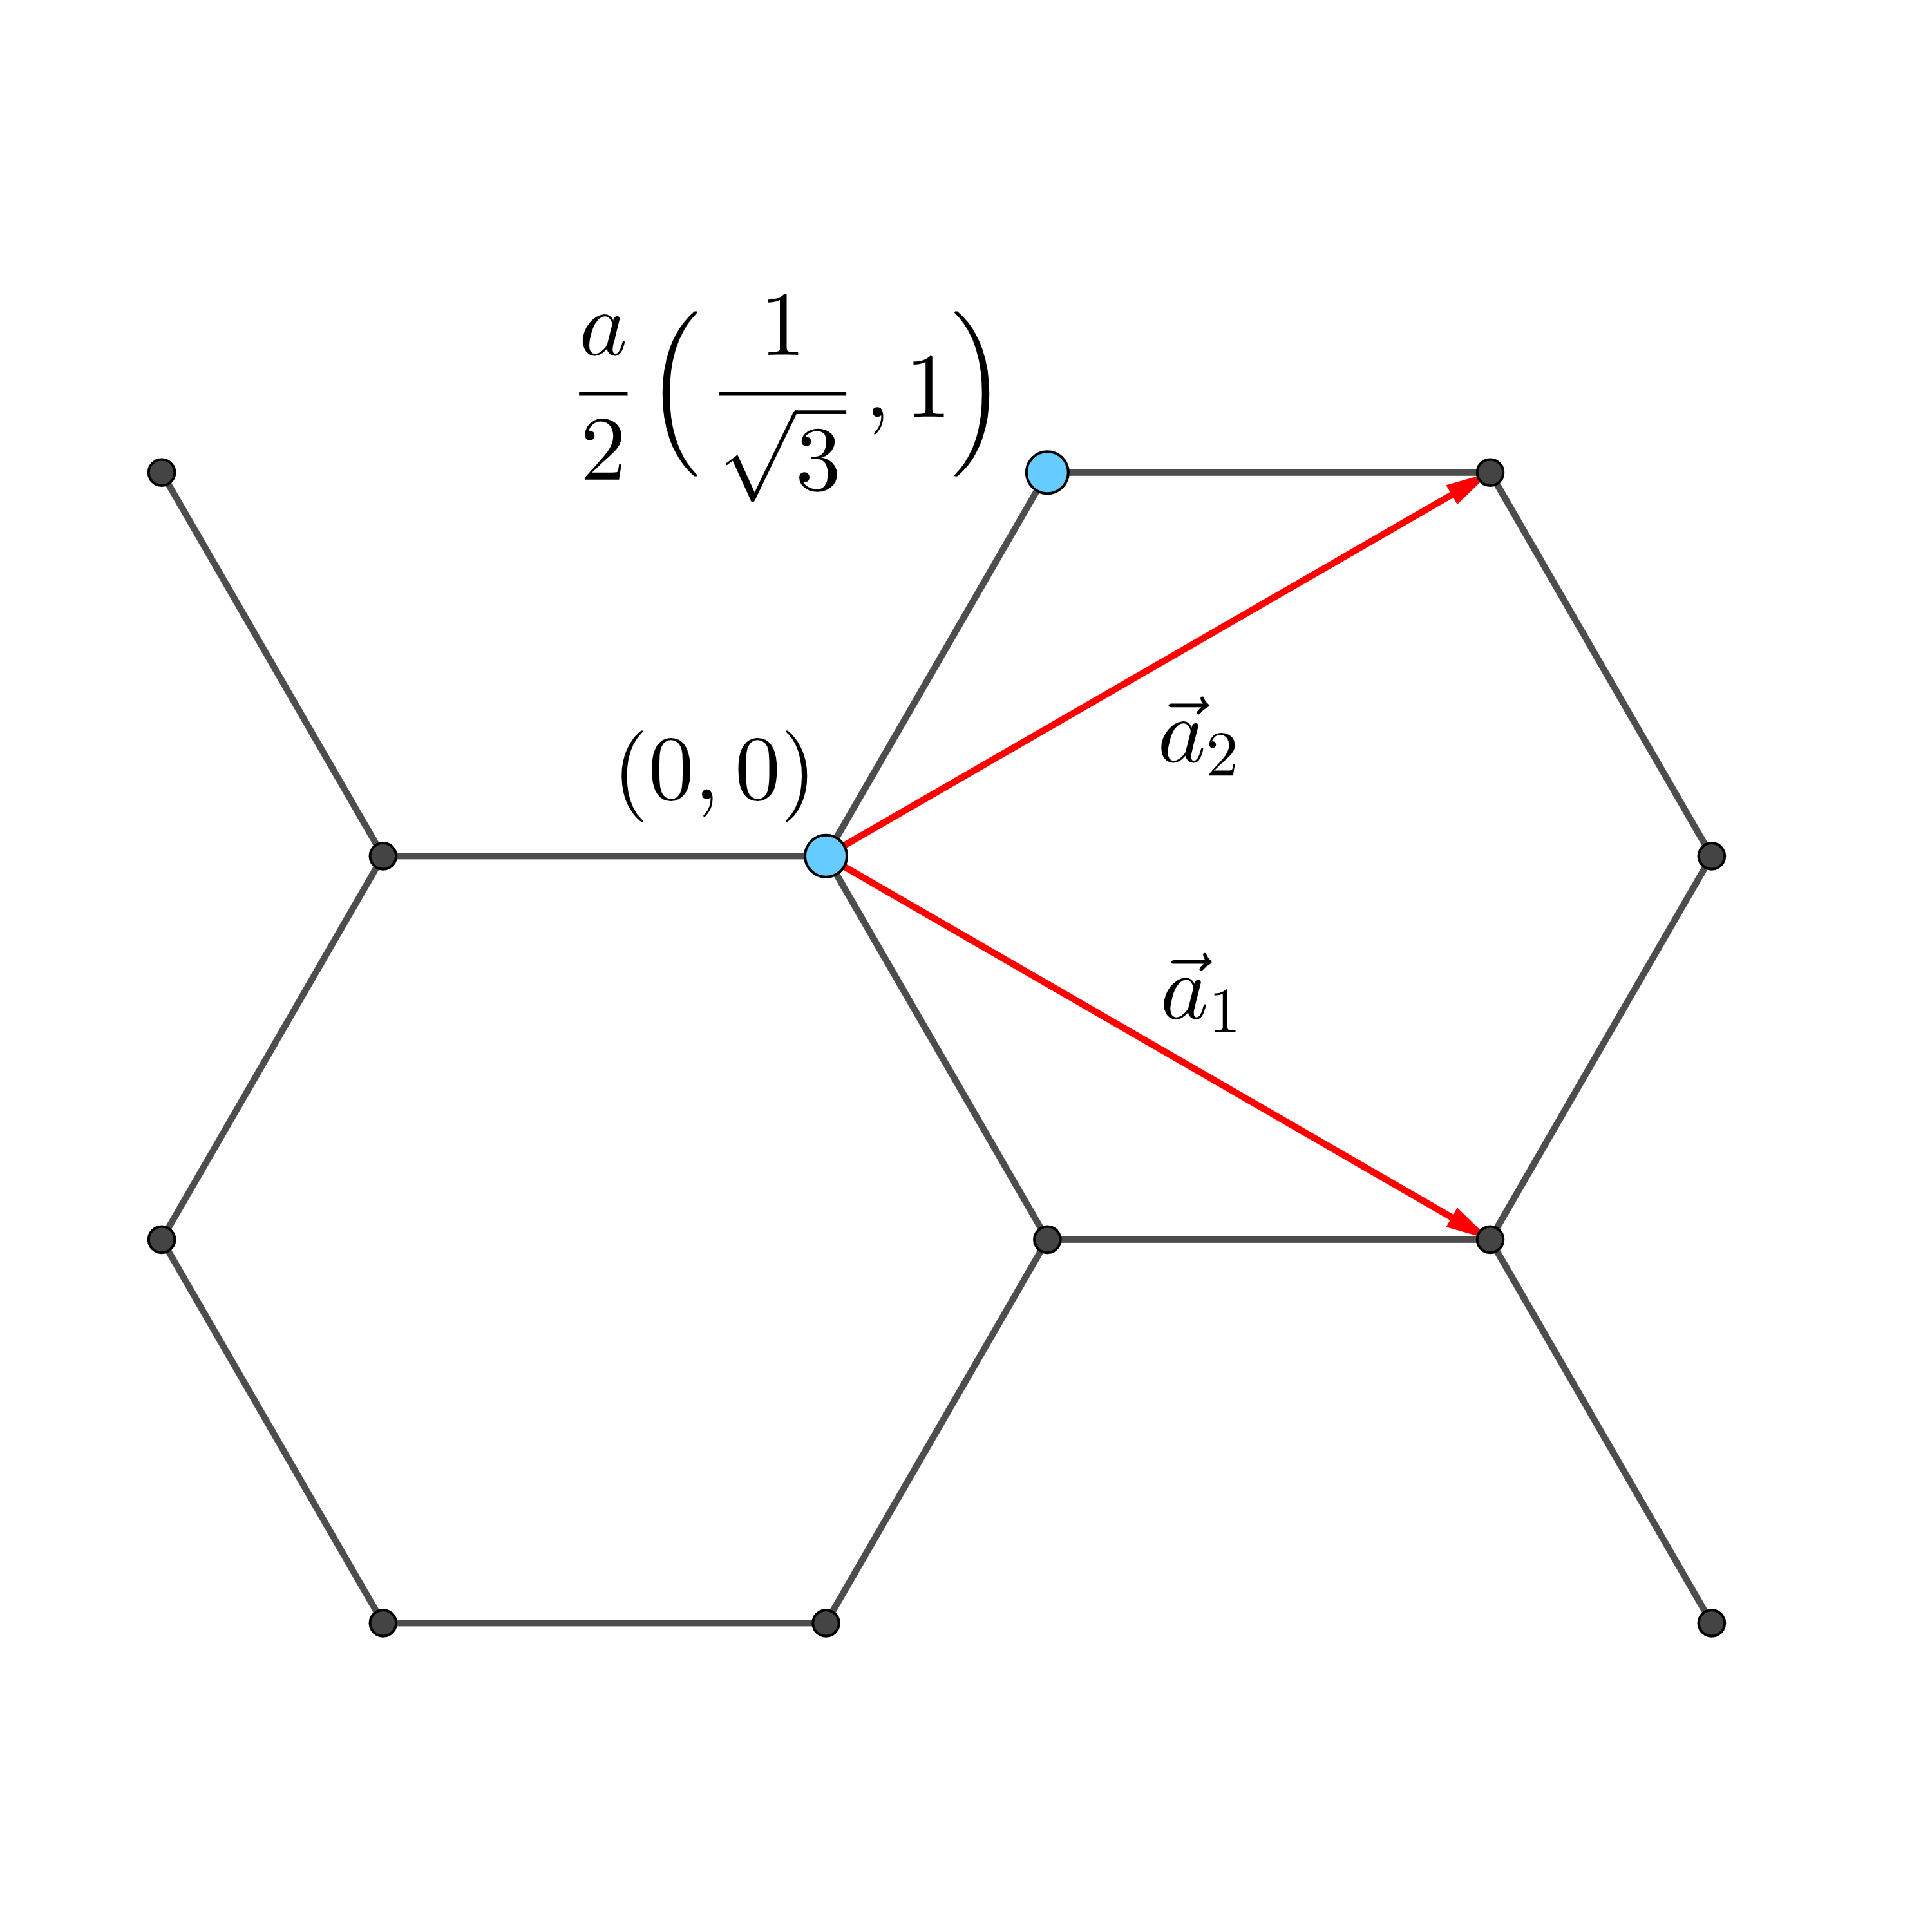
\includegraphics[width=0.3\linewidth]{figures/system/crystal.png}
  \caption{Graphene crystal structure with basis.}
  \label{fig:graphene_crystal}
\end{figure}



\subsection{Indexing}

In order to define the cut patterns applied to the graphene sheet we must define
an indexing system. We must ensure that this gives an unique description of the
atoms as we eventually want to pass a binary matrix, containg 0 for removed atom
and 1 for present atom, that uniquely describes the sheet. We do this by letting
the x-coordinate point to zigzag chains and the y-coordinate to the position
along that chain. This is illustrated in figure \ref{fig:atom_indexing}. Other
solutions might naturally invole the lattice vectors, but as these only can be
used to translate to similar basis atoms a unfortunate duality is introduced as
ones need to include the basis atom of choice into the indexing system. With the
current system we notice that locallity is somewhat preserved. That is, atom
$(i, j)$ is in the proximity of $\{(i+1, j), (i-1, j), (i, j+1), (i, j-1)\}$,
but only three of them is categorized as nearest neighbours due to the hexgonal
structure of the lattice. While $(i, j\pm 1)$ is always nearest neighbours the
neighbour in the x-direction flip sides with incrementing y-coordinate. That is
the nearest neighbours (NN) is decided as
\begin{align*}
  j \ \text{is even} &\rightarrow \text{NN} = \{(i+1, j), (i, j+1), (i, j-1)\}, \\
  j \ \text{is odd} &\rightarrow \text{NN} = \{(i-1, j), (i, j+1), (i, j-1)\}.
\end{align*}

\begin{figure}[H]
  \centering
  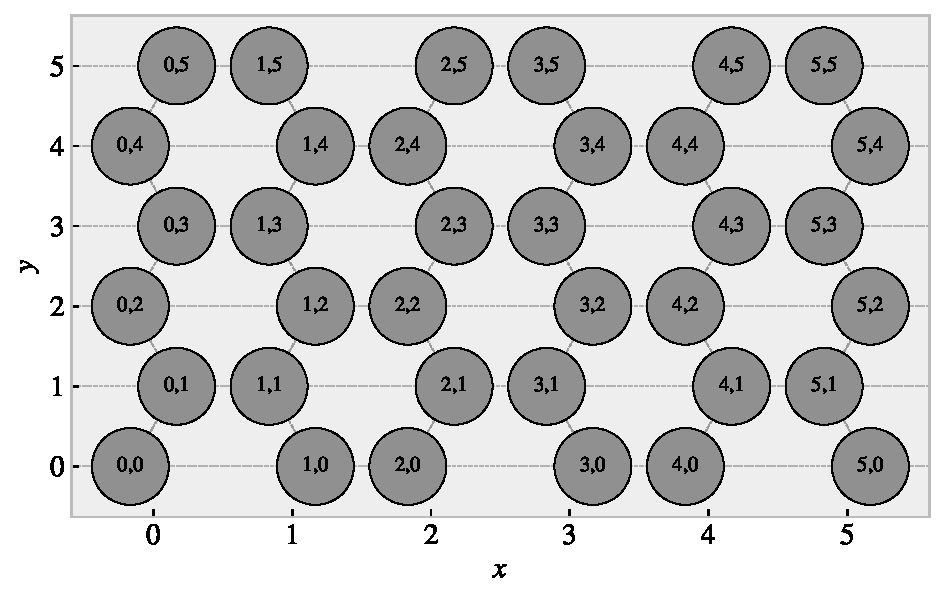
\includegraphics[width=0.7\linewidth]{figures/system/atom_indexing.pdf}
  \caption{Graphene atom indexing}
  \label{fig:atom_indexing}
\end{figure}

\subsection{Removing atoms}

As a mean to ease the formulation of cut patterns we introduce pseudo center
element in each gap of the hexagonal honeycombs, see figure
\ref{fig:center_indexing}. 

\begin{figure}[H]
  \centering
  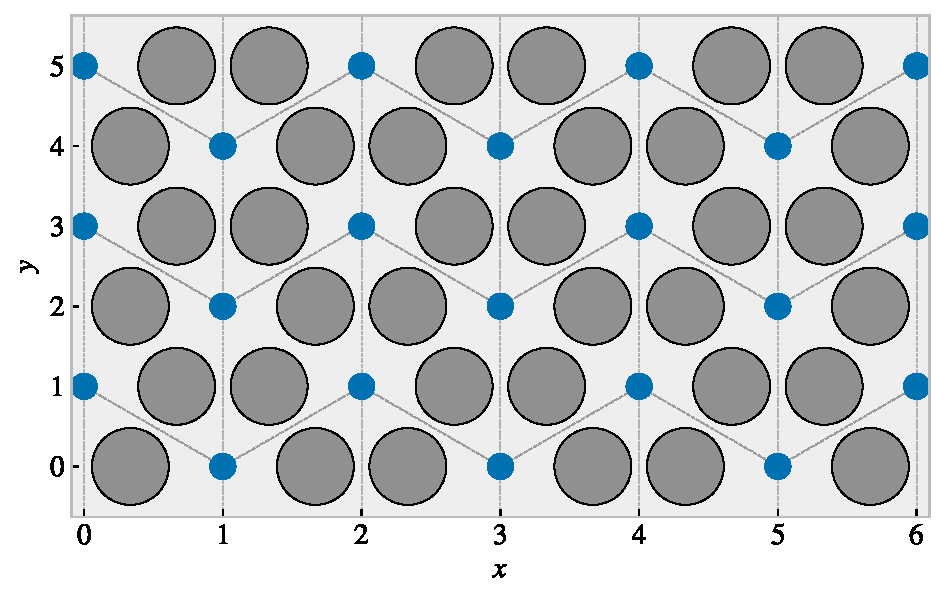
\includegraphics[width=0.7\linewidth]{figures/system/center_indexing.pdf}
  \caption{Graphene center indexing}
  \label{fig:center_indexing}
\end{figure}




Similar to the case of the indexing for the carbon atoms themself the nearest
neighbour center elements alternate with position, this time along the
x-coordinate. Each center element has six nearest neighbours, in clock wise
direction we can denote them: ``up'', ``upper right'', ``lower right'',
``down'', ``lower left'', ``upper left''. The ``up'' and ``down'' is always
accesed as $(i,j\pm 1)$, but for even $i$ the $(i+1,j)$ index corresponds to the
``lower right'' neighbour while for odd $i$ this corresponds to the ``upper
right'' neighbour. This shifting applies for all left or right neighbours and
the full neighbour list is illustrated in figure \ref{fig:center_directions}. 


\begin{figure}[H]
  \centering
  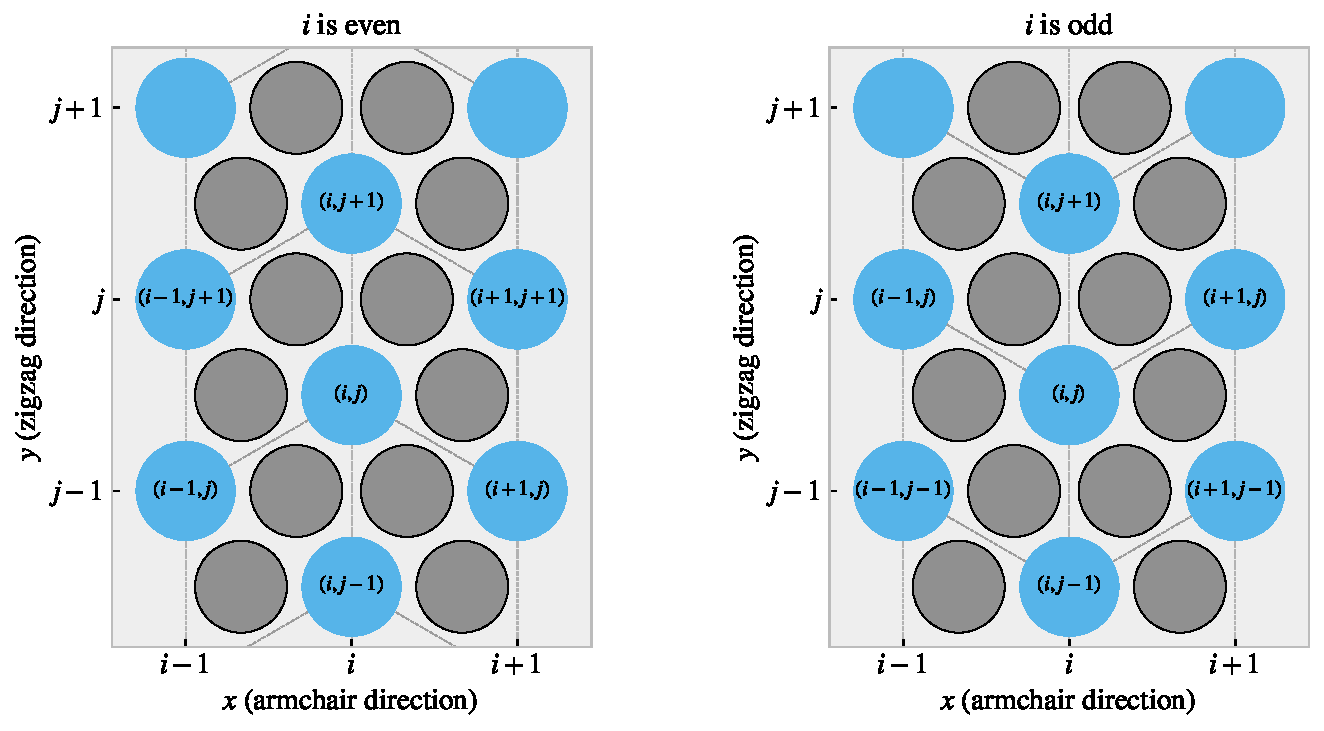
\includegraphics[width=0.7\linewidth]{figures/system/center_directions.pdf}
  \caption{Graphene center elements directions}
  \label{fig:center_directions}
\end{figure}


We define a cut pattern by connecting center elements into connected paths. As
we walk element to element we remove atoms according to one of two rules 
\begin{enumerate}
  \item Remove intersection atoms: We remove the pair of atoms placed directly
  in the path we are walking. That is, when jumnping to the ``up'' center
  element we remove the two upper atoms located in the local hexagon of atoms.
  This method is sensitive to the order of the center elements in the path. 
  \item Remove all surrounding atoms: We simply remove all atoms in the local
  hexagon surrounding each center element. This method is indepdent of the
  ordering of center elements in the path.
\end{enumerate}

We notice that removing atoms using either of these rules will not garuantee an
unique cut pattern. Rule 1 is the more sensitive to paths but we realize that,
for an even $i$, we will remove the same five atoms following either of the
following paths.
\begin{align*}
  (i, j) &\rightarrow \underbrace{(i+1,j+1)}_{\text{upper right}} \rightarrow \underbrace{(i, j+1)}_{\text{up}} \rightarrow \underbrace{(i+1, j+2)}_{\text{upperright + up}} \rightarrow \underbrace{(i+1, j+1)}_{\text{upper right}} \\
  (i, j) &\rightarrow \underbrace{(i+1,j+1)}_{\text{upper right}} \rightarrow \underbrace{(i+1, j+2)}_{\text{upperright + up}} \rightarrow \underbrace{(i, j+1)}_{\text{up}}
\end{align*}

For rule 2 it is even more abovious that different paths can result in the same
atoms being removed. This is the reason that we needed to define and indexing
system for the atom position itself even though that all cuts generated manually
will use the center element path as reference. \\

Illustrate some delete path?



\section{Kirigami patterns}

We propose a series of kirigami inspired cut patterns for the altering of the graphene sheet. We seek inspiration from macroscale patterns that showcases a considerable amount of out of plane buckling when stretched. We choose to imitate two different designs: 1$)$ An alternating repeating series of perpendicular cuts as shown in figure \ref{fig:kirigami_inspiration_a} commonly used in studies of morphable metematerials \cite{new_pop_up}. This patteren produce surface buckling with a tetrahedron (three sided pyramid) shape when stretched. 2$)$ A more intricate pattern shown in figure \ref{fig:kirigami_inspiration_b} which is used Scotch\textsuperscript{TM} Cushion Lock\textsuperscript{TM} \cite{cushion_wrap} as protective wrap for items during shipping. This pattern buckles into a hexagoal honeycomb structure when stretched. In addition to the modeling of the so-called \textit{tetrahedron} and \textit{honeycomb} patterns we also create a series of random walk styled cut patterns.


\begin{figure}[H]
  \centering
  \begin{subfigure}[t]{0.48\textwidth}
      \centering
      \includegraphics[width=\textwidth]{figures/system/pop_up_inspiration.png}
      \caption{}
      \label{fig:kirigami_inspiration_a}
    \end{subfigure}
    \hfill
    \begin{subfigure}[t]{0.48\textwidth}
      \centering
      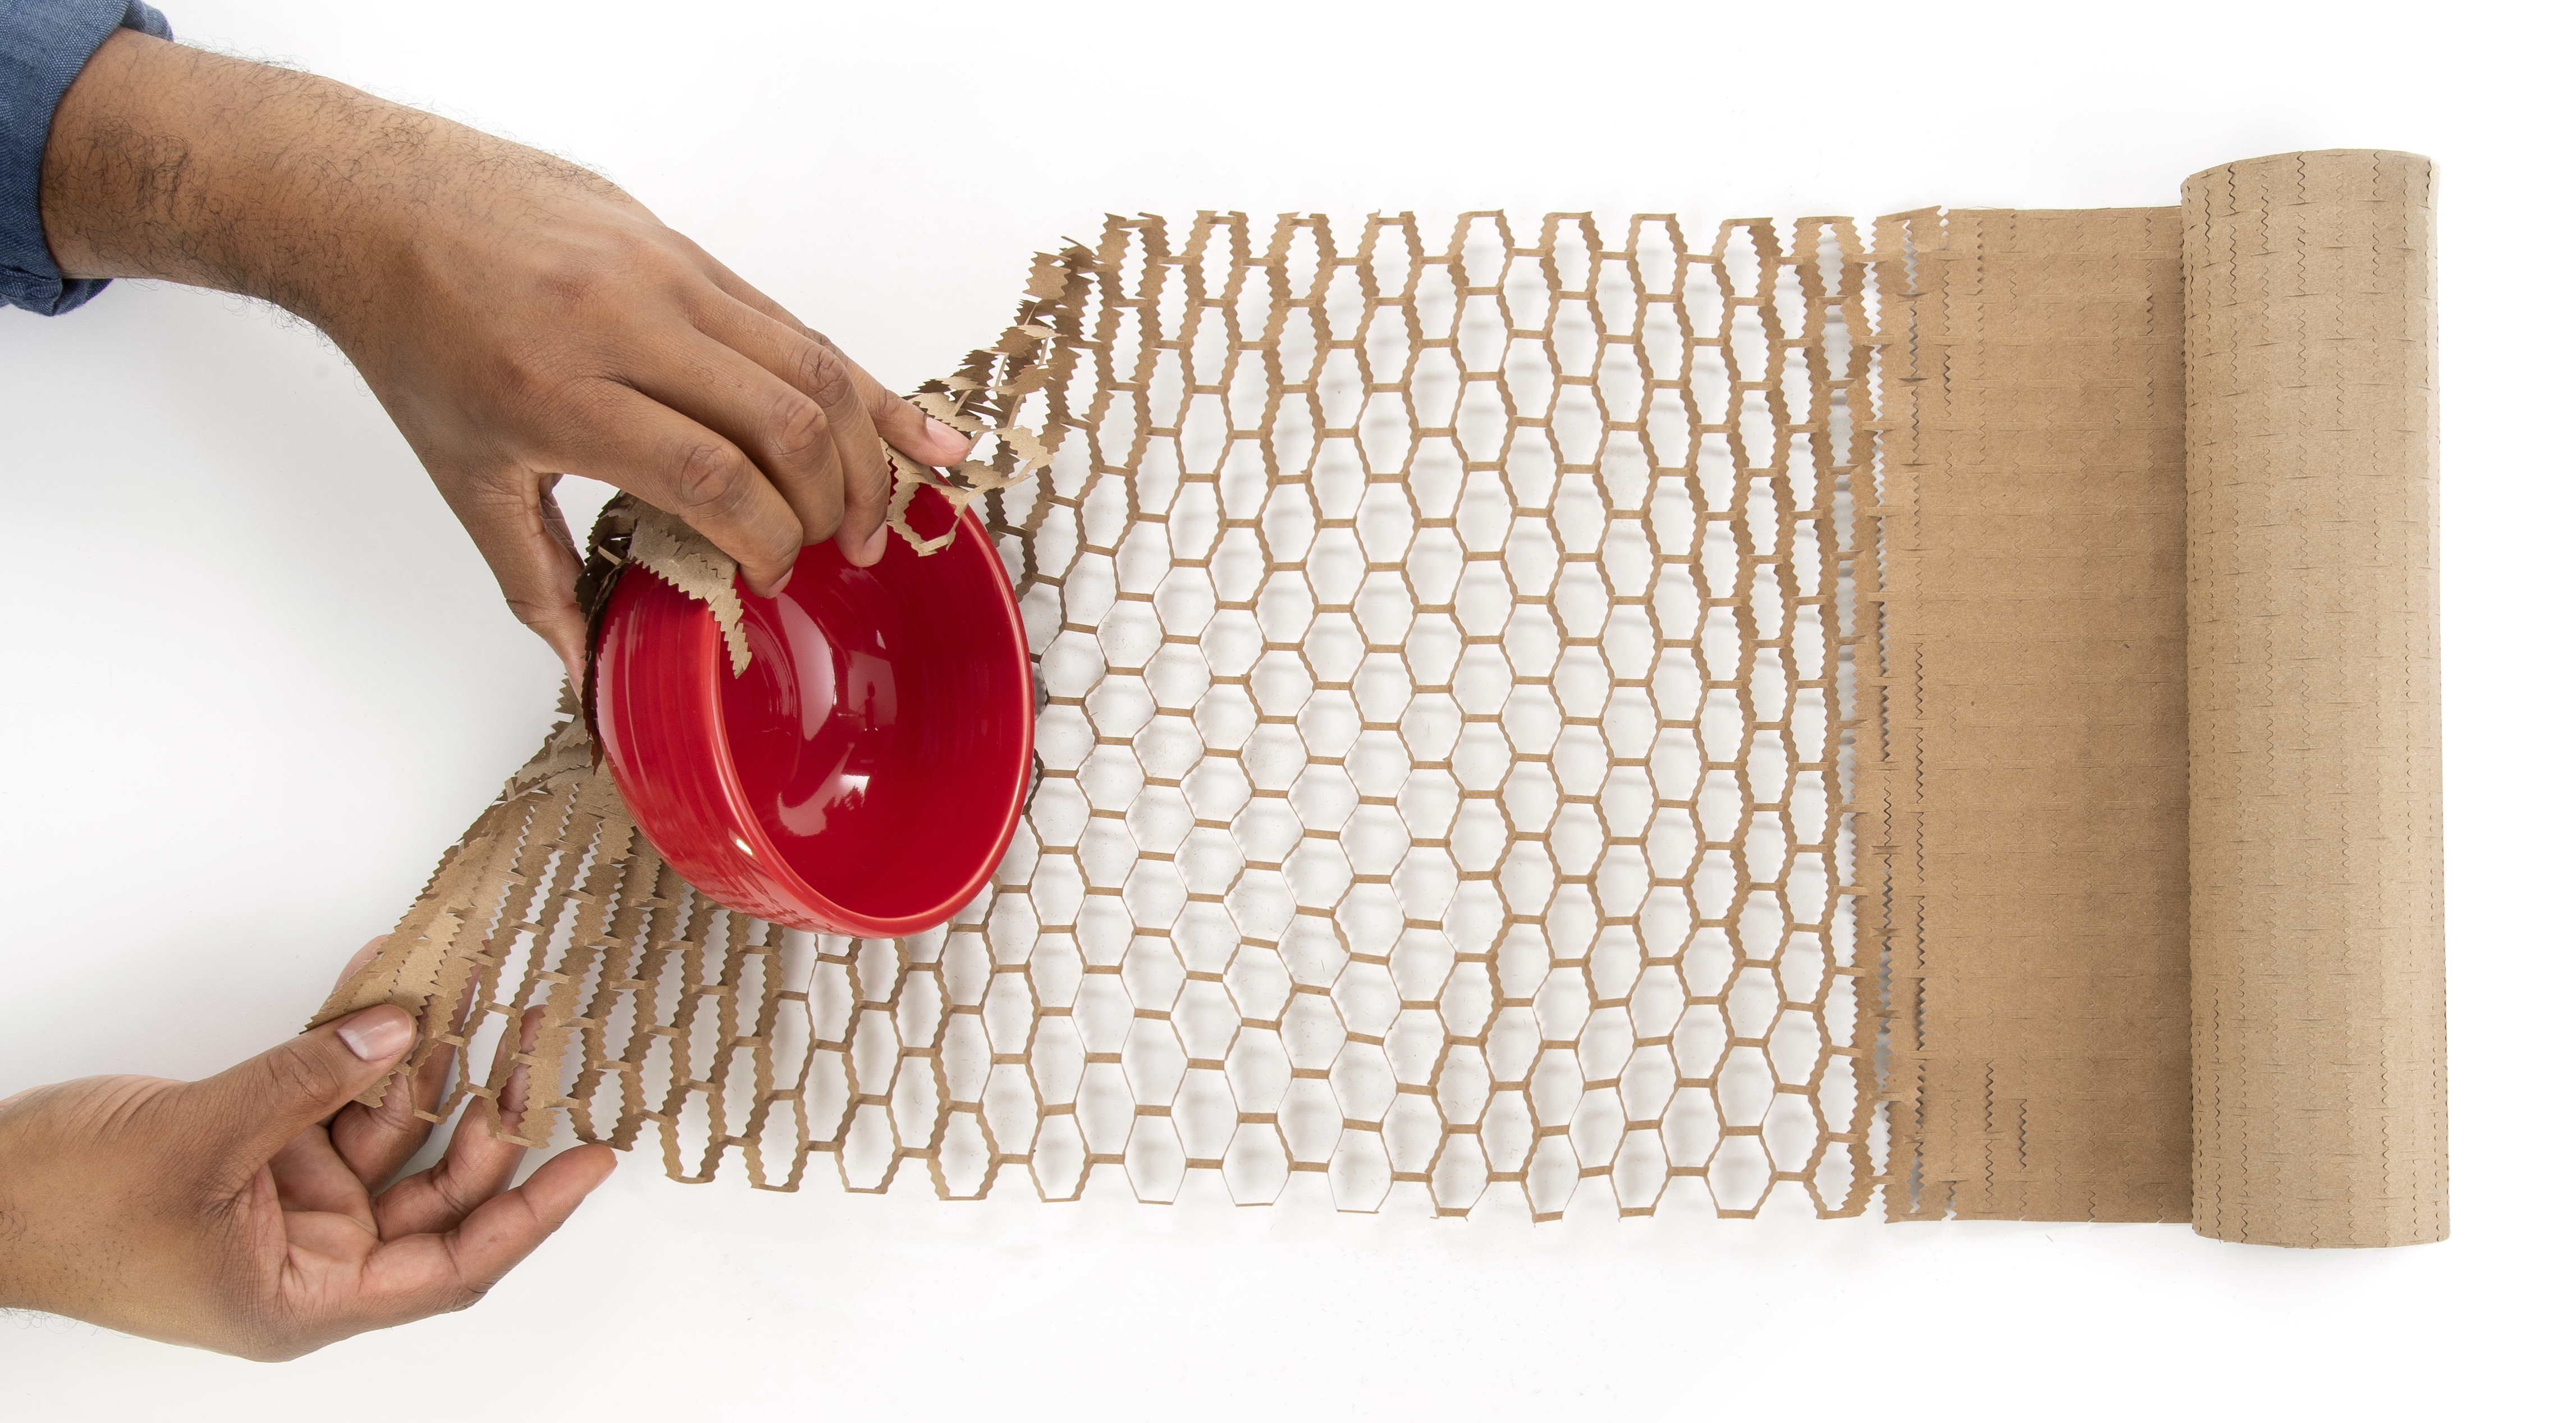
\includegraphics[width=\textwidth]{figures/system/honeycomb_inspiration.jpg}
      \caption{}
      \label{fig:kirigami_inspiration_b}
  \end{subfigure}
  \hfill
     \caption{Macroscale kirigami cut patterns used as inspiraton for the nanoscale implementation. (a) Alternating perpendicular cuts producing a tetrahedron shaped surface buckling when stretched \cite{new_pop_up}. (b) Scotch\textsuperscript{TM} Cushion Lock\textsuperscript{TM} \cite{cushion_wrap} producing a honeycomb shaped surface buckling when stretched.}
     \label{fig:kirigami_inspiration}
\end{figure}

\subsection{Tetrahedron}
The \textit{tetrahedron} pattern is defined in terms of center elements for which all
atoms sourrounding a given center element are removed. The pattern is
characterized by two straight cuts, here denoted line 1 and line 2, arranged
perpendicular to each other such that one line aligns with the center of the
other line and with a given spacing in between. In order to achieve
perpendicular cuts we cannot rely purely on the six principal directions
corresponding to the center element neighbours which is spaced by 60$^\circ$.
Instead, we let line 1 run along the center elemnts in the direction of the
``upper right'' center elements (and ``lower left'') while line 2 goes in the
direction between the ``lower'' and ``lower right'' center elements
corresponding to the direction $(1/\sqrt{3}, -1)$. We define variations of the
pattern by the number of center elements $L_1$ and $L_2$ in line 1 and 2
respectively together with the spacing between the lines $d$ as the tuple $(L_1,
L_2, d)$. The pattern is constructed by translating the two lines to thew whole sheet while according to the spacing. Due to the alignment criterias of having one line point to the center of the other line we can only have odd line length to have a clearly defined center element in the center of each line. Furthermore, in order to ensure that each translated center element stays on the same odd or even type center element we must in practice require that $|L_2 - L_1| = 2, 6, 10, \cdots$. In figure \ref{fig:pop_up} we see a visual representation of the pattern components for the $(7, 5, 2)$ patteren. 


\begin{figure}[H]
  \centering
  \begin{subfigure}[t]{0.48\textwidth}
      \centering
      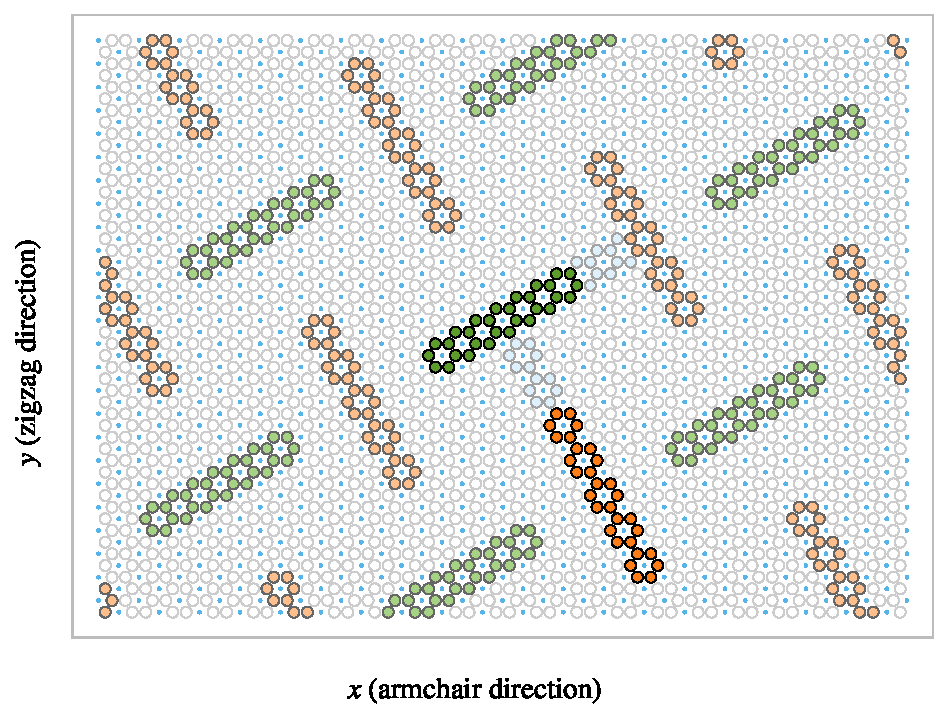
\includegraphics[width=\textwidth]{figures/system/pop_up_inverse.pdf}
      \caption{}
      \label{fig:pop_up_a}
    \end{subfigure}
    \hfill
    \begin{subfigure}[t]{0.48\textwidth}
      \centering
      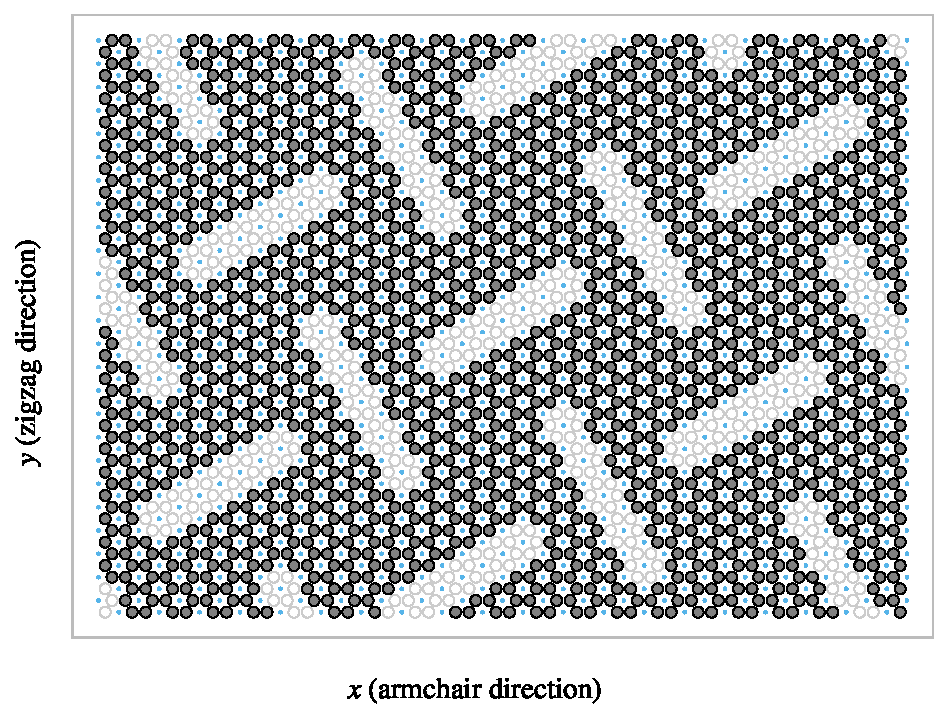
\includegraphics[width=\textwidth]{figures/system/pop_up_pattern.pdf}
      \caption{}
      \label{fig:pop_up_b}
  \end{subfigure}
  \hfill
     \caption{Visual representation of the tetrahedron pattern consisting of two perpendicular lines, line 1 and line 2, of length $L_1$ and $L_2$ respectively with spacing $d$. This example used $(L_1, L_2, d) = (7, 5, 2)$. $(a)$ Highlight of the atoms removed. Line 1 is shown in green and line 2 in orange, with lighter colors for the translated variations, and the spacing is shown in light blue. $(b)$ The sheet after applying the cut pattern where the grey circles denote atoms and the transparent white denotes removed atoms. The small blue circles show the center elements for reference}.
     \label{fig:pop_up}
\end{figure}

In addition to the three parameters $L_1, L_2, d$, the pattern is also anchored to a reference point which describes the position of line 1 and 2 before translating to the whole sheet. Due to the repeating structure of the pattern there exist a small finite number of unique reference positions. For the pattern $(7, 5, 2)$ used as an example in figure \ref{fig:pop_up} there are 140 \footnote{The calculation of this is rather complicated in comparision of the importance in this context. Thus, we exclude the formula for this calculation as the derivation is rather handwavy and the number stated here is numerically backed for this specific parameter set.} Some additional variation of the pattern deviaiton from the example in \ref{fig:pop_up} is showcased in figure \ref{fig:pop_up_flavors}

\begin{figure}[H]
  \centering
  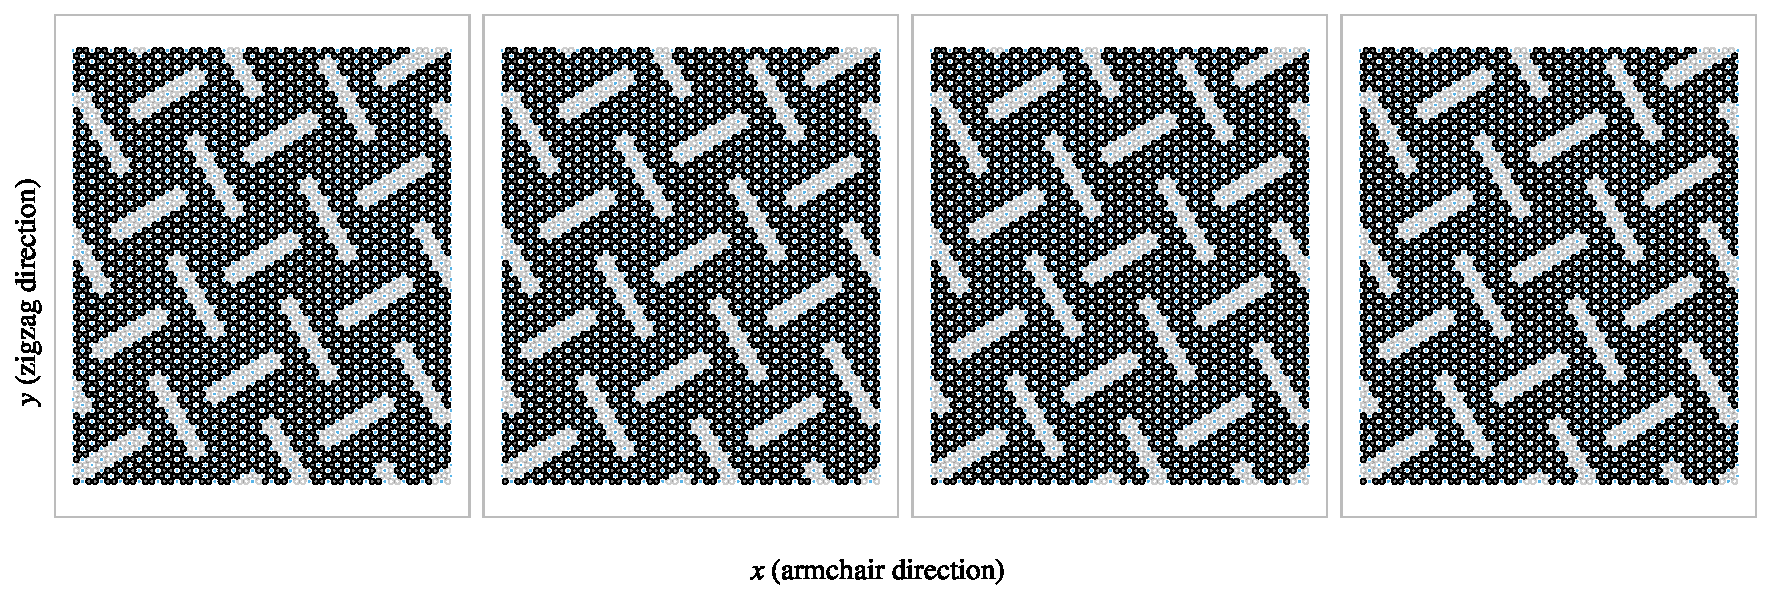
\includegraphics[width=\linewidth]{figures/system/pop_up_flavors.pdf}
  \caption{}
  \label{fig:pop_up_flavors}
\end{figure}



\subsection{Honeycomb}
The \textit{honeycomb} pattern is defined, similarly to the tetrahedron pattern,
in terms of center elements for which all atoms sourrounding a given center
element are removed. The honeycomb pattern is build from a repeating series of
cuts remniscient of a roman numeral one put on its side
(\rotatebox[origin=c]{90}{\MakeUppercase{\romannumeral 1}}). With a given spacing these are put next to each other in the x-direction (\rotatebox[origin=c]{90}{\MakeUppercase{\romannumeral 1}}
\rotatebox[origin=c]{90}{\MakeUppercase{\romannumeral 1}}
\rotatebox[origin=c]{90}{\MakeUppercase{\romannumeral 1}}) to achieve a row
where only a thin \textit{bridge} in between each cut is left to connect the sheet in the y-direction. By placing multiple rows along the y-direction with alternating x-offsett we get the class of honeycomb patterns as visualized in figure \ref{fig:honeycomb}. The pattern
is described in terms of the parameters: (x-width, y-width, bridge thickness,
bridge length) which is annotated in figure \ref{fig:honeycomb_a} where the parameters (2, 2, 1, 5) is used as an example. Some additional variations of the pattern class is showcased in figure \ref{fig:honeycomb_flavors}


\begin{figure}[H]
  \centering
  \begin{subfigure}[t]{0.48\textwidth}
      \centering
      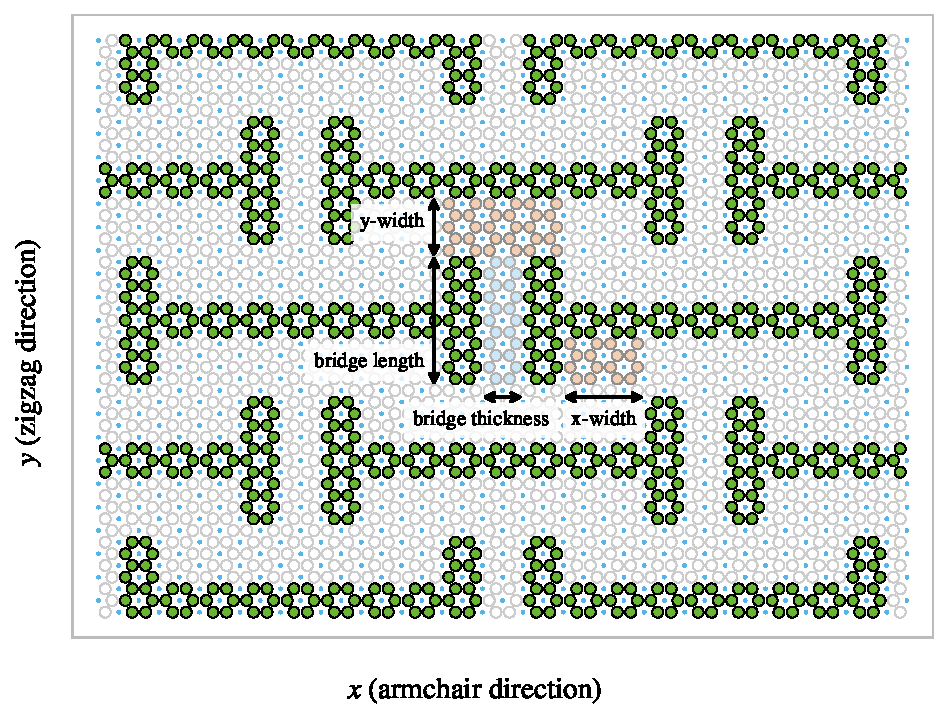
\includegraphics[width=\textwidth]{figures/system/honeycomb_inverse.pdf}
      \caption{}
      \label{fig:honeycomb_a}
    \end{subfigure}
    \hfill
    \begin{subfigure}[t]{0.48\textwidth}
      \centering
      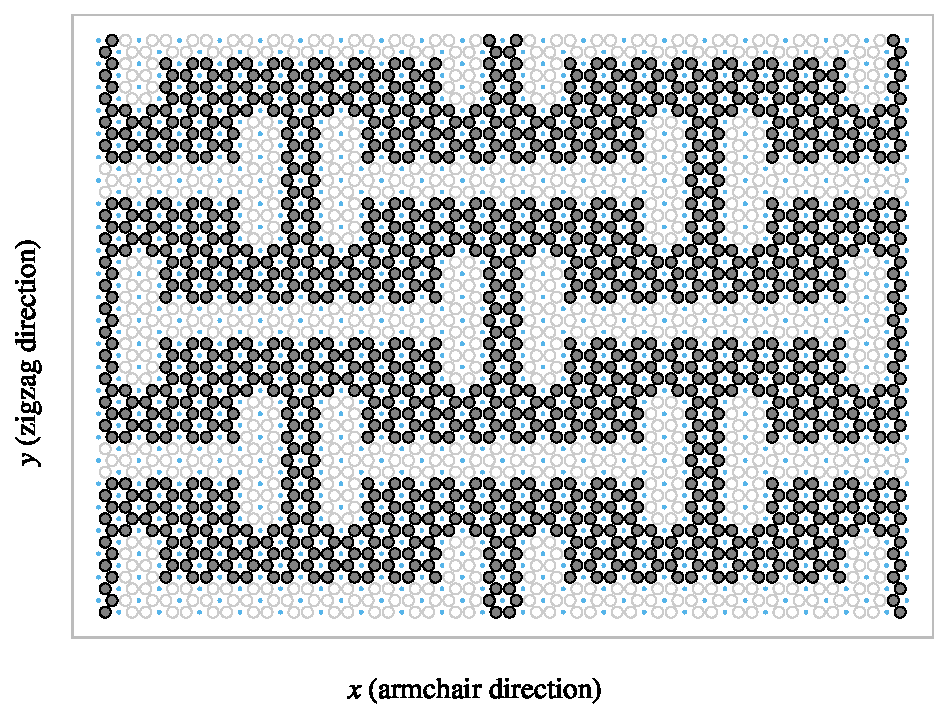
\includegraphics[width=\textwidth]{figures/system/honeycomb_pattern.pdf}
      \caption{}
      \label{fig:honeycomb_b}
  \end{subfigure}
  \hfill
     \caption{}
     \label{fig:honeycomb}
\end{figure}


\begin{figure}[H]
  \centering
  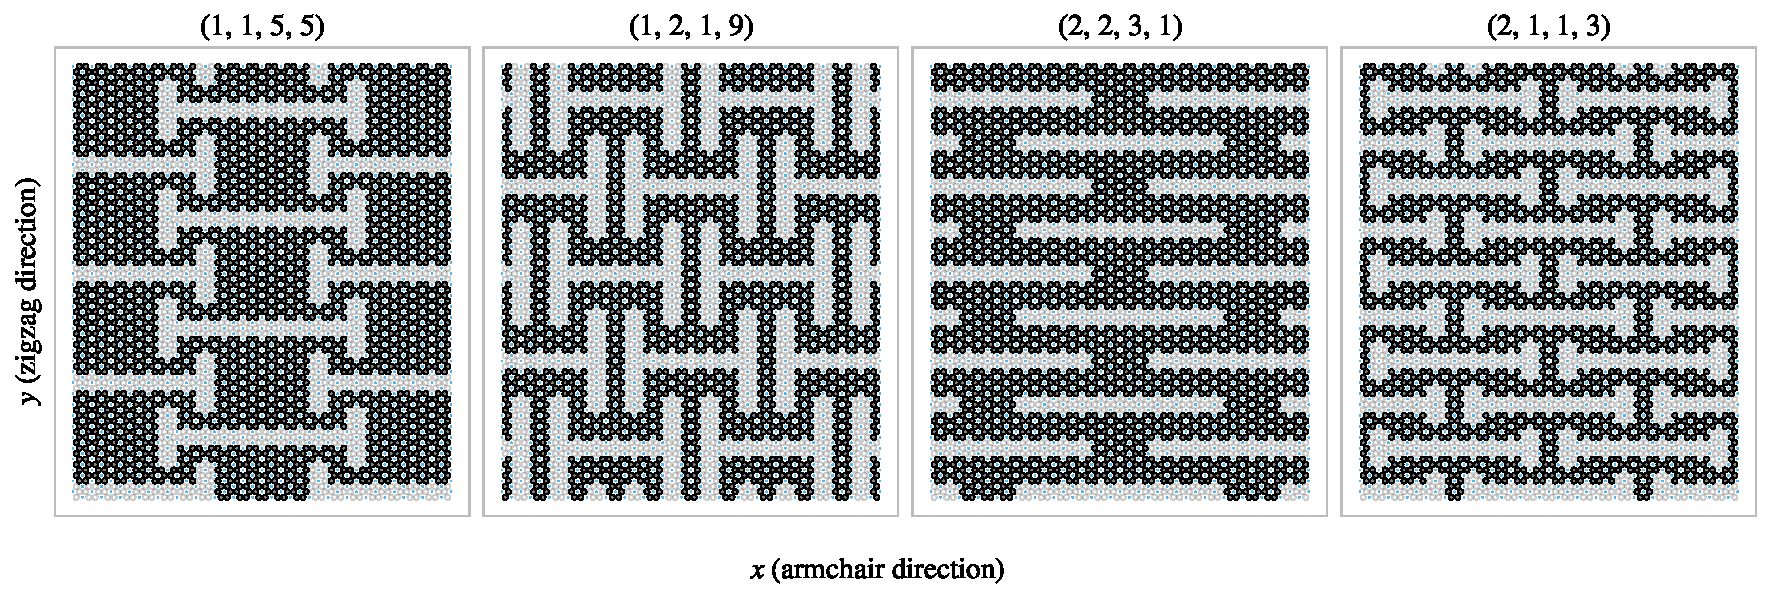
\includegraphics[width=\linewidth]{figures/system/honeycomb_flavors.pdf}
  \caption{}
  \label{fig:honeycomb_flavors}
\end{figure}




\subsection{Random walk}
The random walk serves as a method for introducing random patterns into the dataset with the scope of populating the configuration space more broadly than achieved with the more systematic patterns classes described above. By this argument a more straightforward way to create random configurations could be achieved by random noise, either uniform or gaussian. However, this would often leave the sheet detached with lots of non-connected atom clusters, and intuitively we do not find this promising for the generation of large scale organized structures which is hypothesized to be of interest. The random walk pattern generation is characterized by the parameters summarized in table \ref{tab:RW_params} which will be introduced throughout the following paragraphs. 


\begin{table}[H]
  \begin{center}
  \caption{Parameters for the random walk generator.}
  \label{tab:RW_params}
  \begin{tabular}{ | c | m{12cm} |} \hline
  \textbf{Parameters} & \textbf{Description}  \\ \hline
  Num.\ walkers ($M$)  & Number of random walks to be initiated on the sheet (one at a time). \\ \hline
  Max.\ steps ($S$)  & The maximum steps allowed for any random walker. \\ \hline
  Min.\ distance  & \\ \hline
  Bias  & \\ \hline
  Connection  & Walk between atoms or between center elements (removing all adjecent atoms) \\ \hline
  Avoid unvalid  & \\ \hline
  RN6  & \\ \hline
  grid start  & \\ \hline
  centering  & \\ \hline
  stay or break  & \\ \hline
  avoid clustering  & \\ \hline
  Periodic  & \\ \hline
  \end{tabular}
  \end{center}
\end{table}

\subsubsection{Fundamentals} % M, S, Connection, Periodic, Avoid unvalid
For an uncut sheet we deploy $M$ random walkers one at a time and let them walk
for a maximum number of $S$ steps. We can either let the walker travel between
atom sites, removing the atoms in the path as it goes, or between center
elements, removing all sourrounding atoms - \textit{Connection: Atom/Center
elements}. Nonetheless, we will always remove a site once visited such that the
walker itself or any other walker cannot use this site again. This corresponds
with the property of a self avoiding random walk, but it futhermore constraint
the walkers not to visit any path previously visited by another walker on the
sheet. By default, the walker has an equal chance of chosing any of its adjecent
neighbours for the next step, i.e.\ we draw the next step from a discrete
uniform distribution. Optionally we can use periodic bounary conditions,
\textit{Periodic: True/False}, allowing neighbouring sites to be connected
through the edge in both the x and y-direction. When traveling on atom sites
this gives three nieghbour options for the next step while traveling on the
center elements gives six neighbour options. If the walker happens to arrive at
an already visited site the walk is terminated early. Optionally, we can choose
to remove any neighbouring sites already visited from the neighbour list,
\textit{Avoid unvalid: True/False}, and choose uniformly between the remaining
options instead. This prolongs the walking distance. However, the walker is
still able to find itself in a situation where no neighbouring sites is
availble, note that it cannot backtrack its own path either, and in such a case
the walk is always terminated dispite the setting of \textit{Avoid unvalid}.


\subsubsection{Spacing of walking paths}
In order to control the spacing between the paths of the various walkers we
implement a so-called \textit{minimum distance: 0, 1, \ldots} parameter,
describing the spacing required between paths in terms of the least amount of
steps. When a walker has ended its walk, either by early termination or hitting
the maximum limits of steps, all sites within a walking distance of the minimum
distance is marked as visited, allthough they are not removed from the sheet.
This prevents any subsequent walkers to visit those sites in their walk
according to the general behaviour described in the
previous paragraph. In practice this is done through a recursive algorithm as described in algorithm \ref{algo:walk_dis}. After the walker has ended its walk this function is called for a list of all sites in the path. The function then gatheres gather all sourrounding neighbours regardless of their state on the sheet and call itself using a list of those neighbours. This means that it will follow all possible paths connected to the inital path of inerest. However, this recursiveness terminates when the number of recursive calls exceeds the given minimum distance. The resulting output is then all sites within a walking distance less or equal to the minimum distance which can then be marked as visited. 


\begin{algorithm}[H]
  \caption{Recursive algorithm implemented as class method to mark sites within a distance of the class attribute self.min\_dis.}
  \label{algo:walk_dis}
  \begin{algorithmic}[1]
    \Require self.min\_dis $>$ 0 \Comment{This pseudocode does not handle other cases}
    \Function{walk\_distance}{self, input, dis = 0, pre = [ ]}
      % \State neigh $\gets$ NewList() 
      \State new\_neigh $\gets$ [ ] \Comment{Initialize list for new neighbours}
      \For{site in input}
        \State neigh $\gets$ get\_neighbouring\_sites(site) \Comment{Get sourrounding neighbours}
        \For{n in neigh}
          \If {(n not in pre) and (n not in new\_neigh)} \Comment{If not already added}
            \State AddItem(new\_neigh, n)
          \EndIf
        \EndFor
      \EndFor
      \State dis += 1 \Comment{Increment distance counter}
      \If{dis $\ge$ self.min\_dis} \Comment{Max limit hit}
        \State \Return input + new\_neigh 
      \Else \Comment{Start a new walk from each of the neighbouring sites}
        \State pre $\gets$ input
        \State \Return pre +  self.walk\_distance(new\_neigh, dis, pre)
      \EndIf
    \EndFunction
  \end{algorithmic}
\end{algorithm}



% We have implemented a minimum distance feature for which the walkers cannot visit any
% sites which is equal to or less than a given distance to the path of a previous
% walker. For this, the distance is measured in the least amount of steps between
% a site of interest and the path. In practice this is achieved by keeping an
% additional matrix of the sheet state. After a walker has terminated its run a
% recursive algorithm is utilized to mark all sites within the given walking
% distance to any of the visited sites in the path. This is done by deploying
% walkers for each site which follows each of the possible neighbouring sites
% recursively until the defined deistance is reached. These walkers do not care
% about present or removed site. All sites covered in this procedure is marked as
% visited in the additional sheet state matrix. When a new walker is deployed it
% will then use this matrix for the evaluation of the neighbour state instead which results in the avoidance of these pesudo removed sites. 


% Show figure of the self.visited shadowing 
\subsubsection{Bias}

We include the option for biased random walks as well. We model the system
analog to the canonical ensemble where each microstate $i$ has the associated
probability $p_i$ (Gibbs–Boltzmann distribution) 
\begin{align*}
  p_{i} = \frac{1}{Z}e^{-\beta E_i},
\end{align*}
where $Z$ is the canonical partition function $Z = \sum_i e^{-E_i/k_BT}$, $\beta
= 1/k_B T$ for the boltzmann constant $k_B$ and temperature $T$, and $E_i$ the
energy of microstate $i$. We model the bias as an external force $F$ acting on
the walker, defined by a magnitude and a direction. We define the current site
as having $E = 0$ such that energy associated to the neighbouring sites are
given as the work required to move there. For a step with length and direction
$\vec{s}$ the energy becomes $E_i = -\vec{s}\cdot\vec{F}$. The step length to neighbouring sites will always be equal and by defining the bias magnitude $B = \beta|\vec{F}||\vec{s}|$ we get that the probability for jumping to site $i$ is given by $p_i = Z^{-1}
\exp{(B\hat{\vec{s}}\cdot\hat{\vec{F}})}$, where the hat denotes the unit direction of the vector. We see that the bias magnitude $B$ captures the opposing effects of the magnitide of the external force and the temperature as $B\propto |\vec{F}|/T$. We notice that $\hat{\vec{s}}\cdot\hat{\vec{F}} = \cos{(\theta)}$ for the angle $\theta$ between the vectors which shows that the bias will contribute positively the most when the step direction is allinged with the bias direction ($\theta = 0$), have no contribution for orthogonal direction ($\theta = \pm \pi/2$) and contribute negatively the most when the directions are antiparallel ($\theta = \pi$). This aligns intuitively with our expectations of the bias effect that we wanted. In additon the bias magnitude 

The partition function serves simply as a normalization constant which in practice is initially excluded from the calculation of $p_i$ and then enforced afterwards as a divition by the sum of all $p_i$. In the numerical implementation we then pick the step destination weighted by $p_i$ 


\begin{figure}[H]
  \centering
  \begin{subfigure}[t]{0.48\textwidth}
      \centering
      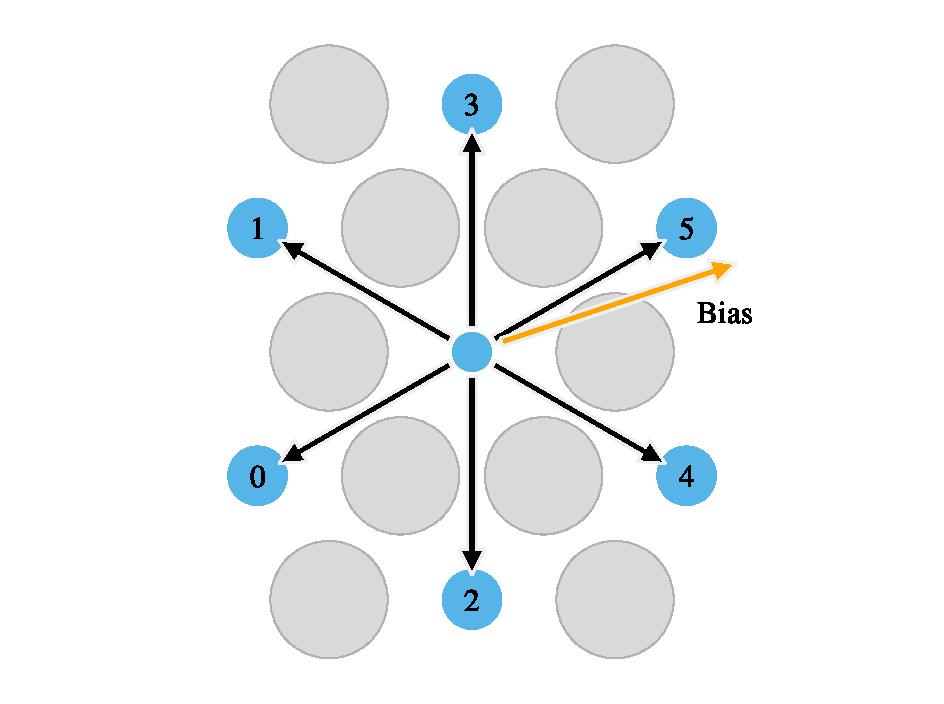
\includegraphics[width=\textwidth]{figures/system/bias_prob_a.pdf}
      \caption{}
      \label{fig:bias_prob_a}
    \end{subfigure}
    \hfill
    \begin{subfigure}[t]{0.48\textwidth}
      \centering
      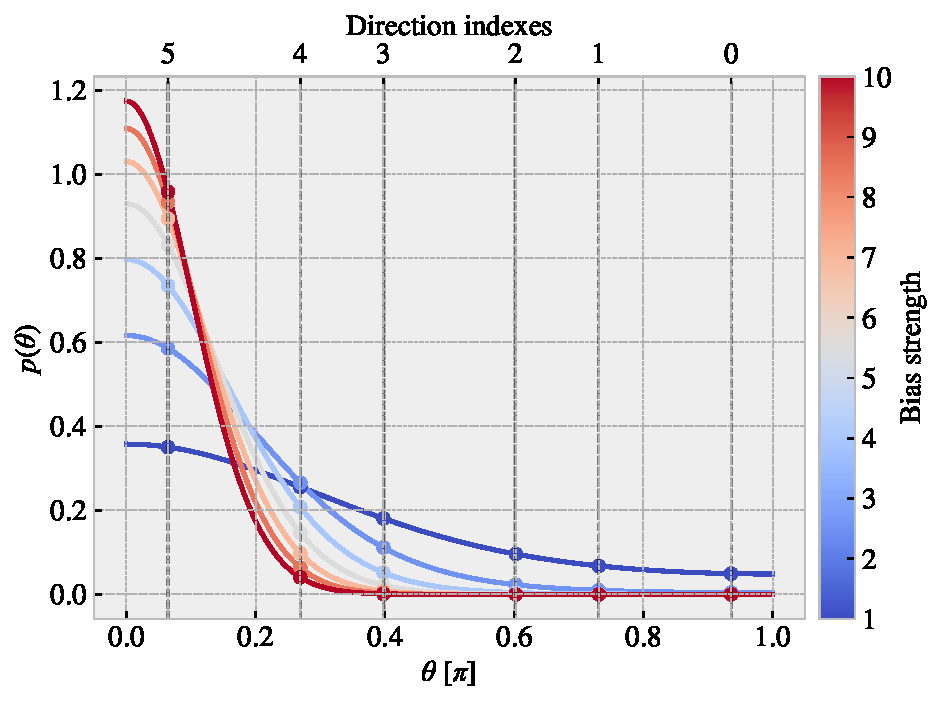
\includegraphics[width=\textwidth]{figures/system/bias_prob_b.pdf}
      \caption{}
      \label{fig:bias_prob_b}
  \end{subfigure}
  \hfill
     \caption{}
     \label{fig:bias_prob}
\end{figure}



\subsubsection{Stay or break}


\subsubsection{Deployment position schemes}





